\begin{figure}[htbp]
\centering
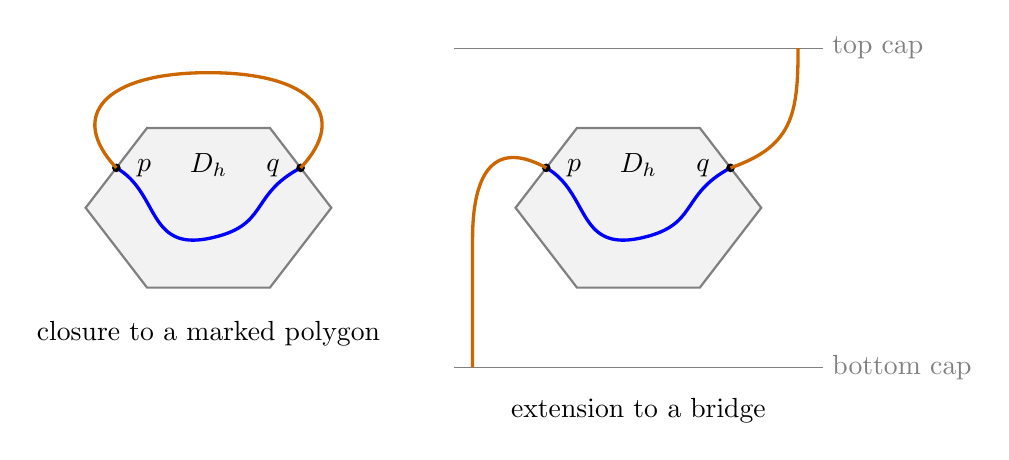
\begin{tikzpicture}[scale=.78,>=stealth]
\foreach \x in {0,7} {
  \begin{scope}[xshift=\x cm]
    \fill[gray!10] (-2,0)--(-1,-1.3)--(1,-1.3)--(2,0)--(1,1.3)--(-1,1.3)--cycle;
    \draw[gray,thick] (-2,0)--(-1,-1.3)--(1,-1.3)--(2,0)--(1,1.3)--(-1,1.3)--cycle;
    \draw[very thick,blue] (-1.5,.65) .. controls (-.8,.25) and (-1,-.7) .. (0,-.5)
      .. controls (1,-.3) and (.65,.2) .. (1.5,.65);
    \fill (-1.5,.65) circle(2pt) node[right=4pt] {$p$};
    \fill (1.5,.65) circle(2pt) node[left=4pt] {$q$};
    \node at (0,.7) {$D_h$};
  \end{scope}
}
\draw[very thick,orange!80!black] (-1.5,.65) .. controls (-2.3,1.5) and (-1.7,2.2) .. (0,2.2)
 .. controls (1.7,2.2) and (2.3,1.5) .. (1.5,.65);
\node at (0,-2.05) {closure to a marked polygon};
\begin{scope}[xshift=7cm]
 \draw[gray] (-3,2.6)--(3,2.6) node[right] {top cap};
 \draw[gray] (-3,-2.6)--(3,-2.6) node[right] {bottom cap};
 \draw[very thick,orange!80!black] (-1.5,.65) .. controls (-2.5,1.2) and (-2.7,.3) .. (-2.7,-.5)--(-2.7,-2.6);
 \draw[very thick,orange!80!black] (1.5,.65) .. controls (2.5,1) and (2.6,1.5) .. (2.6,2.6);
 \node at (0,-3.3) {extension to a bridge};
\end{scope}
\end{tikzpicture}
\caption{The two exterior sewing operations. The blue path is the chord being tested; the orange portions stay outside the convex domain. The proof realizes these schematic curves through pure-direction corridors and varies their intermediate cuts. The two boundary crossings recover the original chord for a fixed cut choice.}
\label{fig:sewing}
\end{figure}
